\chapter{平面几何与空间几何}
古希腊的欧几里得在公元前300年左右写出了旷古烁今的一本书,这就是《几何原本》.
这本书的重要意义不仅体现在它记载了古希腊数学那丰厚的成果,更体现在它提出的欧式几何公理体系以及其后的公理化方法.

\section{欧式公理体系}
\subsection{几何元素}
\begin{definition}\label{definition:欧式几何.几何元素.基本几何元素}
在平面几何中,有两种基本研究对象:
\begin{enumerate}
\item \textbf{点}(我们常用大写拉丁字母\(A,B,C,\dotsc\)表示);
\item \textbf{直线}(我们常用小写拉丁字母\(a,b,c,\dotsc\)表示).
\end{enumerate}
在空间几何中,除了上述两种以外,还多了一种研究对象:
\begin{enumerate}
\setcounter{enumi}{2}
\item \textbf{平面}(我们常用小写希腊字母\(\alpha,\beta,\gamma,\dotsc\)表示).
\end{enumerate}
点和直线统称为“平面几何的\textbf{元素}”;
点、直线和平面统称为“空间几何的\textbf{元素}”.
\end{definition}

我们设想,点、直线、平面这三类几何元素之间总是存在某种关系.
根据这些关系,我们提出以下五组命题,并认定它们恒为真,特别地称它们为“公理(axiom)”.

\subsection{第一组公理:关联公理}
本组公理是在前面提到的点、直线和平面这三类几何元素之间建立联系,其条文如下.
\begin{axiom}[关联公理]\label{axiom:欧式几何.关联公理}
点、直线和平面这三类几何元素存在如下的关系:
\begin{enumerate}
\item 对于两点\footnote{%
在本章中,当提到“两点”“两条直线”等时,都是指两个相异的几何元素.%
}\(A\)和\(B\),%
恒有一直线\(l\),%
它同\(A\)和\(B\)这两点的每一点都相关\footnote{%
同一种关系可能存在多种说法,%
例如“直线\(l\)同\(A\)和\(B\)这两点的每一点都相关”
可以说成是“直线\(l\)通过点\(A\)、点\(B\)”
或“直线\(l\)连结点\(A\)和点\(B\)”,%
而“点\(A\)与直线\(l\)相关”可以说成是“点\(A\)在直线\(l\)上”
“点\(A\)是直线\(l\)(上)的一点”或“直线\(l\)含有点\(A\)”.%
“点\(P\)既在直线\(a\)上,%
又在直线\(b\)上”可以说成是“点\(P\)是直线\(a\)和直线\(b\)的\textbf{交点}或\textbf{公共点}”
或“直线\(a\)、\(b\)相交于点\(P\)”.
}.

\item 对于两点\(A\)和\(B\),%
至多有一直线\footnote{%
除了可以用某个小写拉丁字母表示直线以外,与点\(A\)、\(B\)相关的直线还可以记作\(AB\).%
},它同\(A\)和\(B\)这两点的每一点都相关.

\item 一直线上恒至少有两点;至少有三点不在同一直线上.

\item 对于不在同一直线上的任意三点\(A\)、\(B\)和\(C\),恒有一平面\(\gamma\),它同\(A\)、\(B\)和\(C\)这三点的每一点相关;对于任一平面,恒有一点同这平面相关\footnote{%
“点\(A\)与平面\(\gamma\)相关”可以说成是“点\(A\)在\(\gamma\)上”或“点\(A\)是\(\gamma\)的点”.%
}.

\item 对于不在同一直线上的三点\(A\)、\(B\)和\(C\),至多有一平面\footnote{%
除了可以用某个小写希腊字母表示平面以外,由点\(A\)、\(B\)和\(C\)确定的平面还可以记作\(ABC\).%
},它同\(A\)、\(B\)和\(C\)这三点的每一点相关.

\item 若一直线\(l\)的两点\(A\)和\(B\)在一平面\(\gamma\)上,则\(l\)的每一点都在平面\(\gamma\)上\footnote{%
或者说“直线\(l\)在平面\(\gamma\)上”.%
}.

\item 若两平面\(\alpha\)和\(\beta\)有一个公共点\(A\),则它们至少还有一个(与\(A\)相异的)公共点\(B\)\footnote{%
这表明空间的维数不大于3.%
}.

\item 至少有四点不在同一平面上\footnote{%
这表明空间的维数不小于3.%
}.
\end{enumerate}
\end{axiom}
\cref{axiom:欧式几何.关联公理} 的前3个命题可以统称为\textbf{平面公理},后5个命题可以统称为\textbf{空间公理}.

依据\cref{axiom:欧式几何.关联公理} 可以推证出以下两条定理.
\begin{theorem}\label{theorem:欧式几何.定理1}
一平面上的两直线或有一公共点,或无公共点;
两平面或无公共点,或有一公共直线;
两平面无公共直线时无公共点;
一平面和不在其上的一直线或无公共点,或有一公共点.
\end{theorem}

\begin{theorem}\label{theorem:欧式几何.定理2}
过一直线和不在这直线上的一点,或过有公共点的两条不同直线,恒有一个而且只有一个平面.
\end{theorem}

\subsection{第二组公理:顺序公理}
本组公理规定了“介于”(或“在……之间”)这个概念.
根据这个概念,直线上的、平面上的和空间中的点才有顺序可言.
\begin{axiom}[顺序公理I]\label{axiom:欧式几何.顺序公理1}
在一直线上的点有一定的相互关系.
我们特别用“介于”(或“在……之间”)来描述它.
\begin{enumerate}
\item 若一点\(B\)在一点\(A\)和一点\(C\)之间(如\cref{figure:欧式几何.直线上点的顺序1} ),则\(A\)、\(B\)和\(C\)是一直线上的不同的三点,同时\(B\)也在\(C\)和\(A\)之间.
\begin{figure}[ht]
\centering
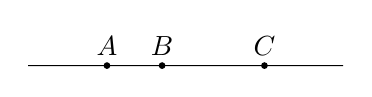
\begin{tikzpicture}
\draw[fill=black] (0,0)--(1,0)node[above]{\(A\)}circle(1pt)
--(1.7,0)node[above]{\(B\)}circle(1pt)
--(3,0)node[above]{\(C\)}circle(1pt)
--(4,0);
\end{tikzpicture}
\caption{直线上点的顺序}
\label{figure:欧式几何.直线上点的顺序1}
\end{figure}

\item 对于两点\(A\)和\(B\)(如\cref{figure:欧式几何.直线上点的顺序2} ),直线\(AB\)上恒至少有一点\(C\),使得\(B\)在\(A\)和\(C\)之间.
\begin{figure}[ht]
\centering
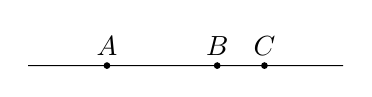
\begin{tikzpicture}
\draw[fill=black] (0,0)--(1,0)node[above]{\(A\)}circle(1pt)
--(2.4,0)node[above]{\(B\)}circle(1pt)
--(3,0)node[above]{\(C\)}circle(1pt)
--(4,0);
\end{tikzpicture}
\caption{直线上点的顺序}
\label{figure:欧式几何.直线上点的顺序2}
\end{figure}

\item 一直线的任意三点中,至多有一点在其他两点之间.
\end{enumerate}
\end{axiom}

在上述三条\textbf{直线顺序公理}之外,还需要一条\textbf{平面顺序公理}.

\begin{axiom}[顺序公理II]\label{axiom:欧式几何.顺序公理2}
考虑一直线\(l\)上的两点\(A\)和\(B\).
我们把这一对点\(A\)和\(B\)确定的介于它们的点的集合叫做一条\textbf{线段},记作\(AB\)(或\(BA\)).
在\(A\)和\(B\)之间的点叫做线段\(AB\)的点,或线段\(AB\)的\textbf{内点};
\(A\)和\(B\)叫做线段\(AB\)的\textbf{端点};
直线\(l\)上的其他点叫做线段\(AB\)的\textbf{外点}.
\begin{enumerate}
\setcounter{enumi}{3}
\item 设\(A\)、\(B\)和\(C\)是不在同一直线上的三点,\(l\)是平面\(ABC\)上的一直线,但\(l\)不通过\(A,B,C\)这三点中的任一点(如\cref{figure:欧式几何.平面上点的顺序1} ),若直线\(l\)通过线段\(AB\)的一点,则它必定也通过线段\(AC\)或线段\(BC\)的一点.
\begin{figure}[ht]
\centering
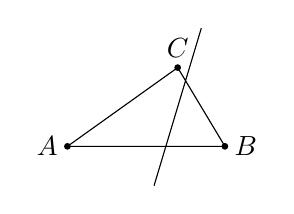
\begin{tikzpicture}
\draw[fill=black] (-1,0)node[left]{\(A\)}circle(1pt)
--(1,0)node[right]{\(B\)}circle(1pt)
--(.4,1)node[above]{\(C\)}circle(1pt)--(-1,0)
(.1,-.5)--(.7,1.5);
\end{tikzpicture}
\caption{平面上点的顺序}
\label{figure:欧式几何.平面上点的顺序1}
\end{figure}
\end{enumerate}
\end{axiom}
直观地说,\cref{axiom:欧式几何.顺序公理2} 说的就是:若一直线“冲进”一个三角形的内部,它必定还要再“冲出”这个三角形.
易证:与线段\(AB\)相交的直线\(l\)不同时和\(AC,BC\)这两条线段都相交.

\subsection{关联公理和顺序公理的推论}
从\cref{axiom:欧式几何.关联公理,axiom:欧式几何.顺序公理1,axiom:欧式几何.顺序公理2} 能推证下列定理.
\begin{theorem}\label{theorem:欧式几何.定理3}
对于两点\(A\)和\(C\),直线\(AC\)上恒至少有一点\(D\),在\(A\)和\(C\)之间.
\begin{proof}
根据\cref{axiom:欧式几何.关联公理} 第3条,直线\(AC\)外存在一点\(E\);
根据\cref{axiom:欧式几何.顺序公理1} 第2条,直线\(AE\)上有一点\(F\),使得\(E\)在线段\(AF\)内.
根据\cref{axiom:欧式几何.顺序公理1} 第2条、第3条,直线\(FC\)上有一点\(G\),不在线段\(FC\)内.
根据\cref{axiom:欧式几何.顺序公理2} 第4条,直线\(EG\)必交线段\(AC\)于一点\(D\).
\end{proof}
\end{theorem}

\begin{theorem}\label{theorem:欧式几何.定理4}
一直线上的任意三点\(A,B,C\)中,必有一点且只有一点在其他两点之间.
\begin{proof}
设\(A\)不在\(B\)和\(C\)之间,而且\(C\)不在\(A\)和\(B\)之间.
用直线连接\(B\)和直线\(AC\)外一点\(D\).
根据\cref{axiom:欧式几何.顺序公理1} 第2条,能在直线\(BD\)上取一点\(G\),使得\(D\)在\(B\)和\(G\)之间.
对于三角形\(BCG\)和直线\(AD\)应用\cref{axiom:欧式几何.顺序公理2} 第4条,可知直线\(AD\)通过线段\(CG\)内的一点\(E\);
同理可知直线\(CD\)通过线段\(AG\)内一点\(F\).
对于三角形\(AEG\)和直线\(CF\)应用\cref{axiom:欧式几何.顺序公理2} 第4条,可知\(D\)在\(A\)和\(E\)之间;
再对于三角形\(AEC\)和直线\(BG\)应用\cref{axiom:欧式几何.顺序公理2} 第4条,即证得\(B\)在\(A\)和\(C\)之间.
\end{proof}
\end{theorem}

\begin{theorem}\label{theorem:欧式几何.定理5}
一直线上的任意四点\(A,B,C,D\),使得点\(B\)既在\(A\)和\(C\)之间,又在\(A\)和\(D\)之间;
而且点\(C\)既在\(A\)和\(D\)之间,又在\(B\)和\(D\)之间.
\end{theorem}

\begin{corollary}\label{theorem:欧式几何.定理6}
一直线上的任意有限个点\(A,B,C,\dotsc,K\),%
使得点\(B\)在\(A\)和\(C\),或和\(D\),或和\(E\),……,或和\(K\)之间;
而且点\(C\)在\(A\)(或\(B\))和\(D\),或和\(E\),……,或和\(K\)之间;以此类推.
\end{corollary}

\begin{corollary}\label{theorem:欧式几何.定理7}
一直线上任意两点之间恒有无限多个点.
\end{corollary}

\begin{theorem}\label{theorem:欧式几何.定理8}
一平面\(\gamma\)上的任一直线\(l\)将该平面上其余的点分为具有下述性质的两个区域:
一个区域的任一点\(A\)与另一区域的任一点\(B\)所决定的线段\(AB\)内,%
必含有直线\(l\)的一点(如\cref{figure:欧式几何.直线l分平面为两个区域} );%
而同一个区域的任意两点\(A\)和\(A'\)所决定的线段\(AA'\)内,不含有直线\(l\)的点.
\begin{figure}[ht]
\centering
\begin{tikzpicture}
\draw (-2,0)--(2,0)node[right]{\(l\)}
(.5,-1)node[right]{\(B\)}--(-.5,.5)node[left]{\(A\)}--(.3,1)node[right]{\(A'\)};
\end{tikzpicture}
\caption{直线\(l\)分平面为两个区域}
\label{figure:欧式几何.直线l分平面为两个区域}
\end{figure}
\end{theorem}

\begin{definition}
我们说\(A\)和\(A'\)这两点在平面\(\gamma\)上直线\(l\)的\textbf{同侧}%
(如\cref{figure:欧式几何.直线l分平面为两个区域} ),%
而\(A\)和\(B\)这两点在平面\(\gamma\)上直线\(l\)的\textbf{异侧}.%
\end{definition}

\begin{definition}
设\(A,A',O\)和\(B\)是一直线\(l\)上的四点(如\cref{figure:欧式几何.射线} ),%
而\(O\)在\(A\)和\(B\)之间,但不在\(A\)和\(A'\)之间.
我们称“\(A\)和\(A'\)这两点在\(l\)上点\(O\)的\textbf{同侧}”,%
而称“\(A\)和\(B\)这两点在\(l\)上点\(O\)的\textbf{异侧}”.

直线\(l\)上点\(O\)的同侧的点的全体,叫做从点\(O\)起始的一条\textbf{射线};
因此一直线的每一点把这直线分成两条射线.
\begin{figure}[ht]
\centering
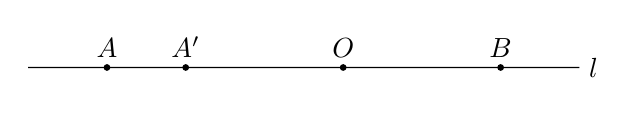
\begin{tikzpicture}
\draw[fill=black] (-3,0)--(-2,0)node[above]{\(A\)}circle(1pt)
--(-1,0)node[above]{\(A'\)}circle(1pt)
--(1,0)node[above]{\(O\)}circle(1pt)
--(3,0)node[above]{\(B\)}circle(1pt)--(4,0)node[right]{\(l\)};
\end{tikzpicture}
\caption{射线}
\label{figure:欧式几何.射线}
\end{figure}
\end{definition}

\begin{definition}
若干条首尾相连的线段\(AB,BC,CD,\dotsc,KL\)的集合叫做一条\textbf{折线段},%
它连结\(A\)和\(L\)这两点.
为求简便,可将这条折线段记为\(ABCD \dotso KL\).
线段\(AB,BC,CD,\dotsc,KL\)的内点和端点都叫做这条折线段的点.
点\(A\)和点\(L\)称为“折线段的\textbf{端点}”.

若折线段\(ABCD \dotso KL\)的顶点\(A,B,C,D,\dotsc,K,L\)都在同一平面上,%
且它的端点\(L\)和\(A\)是同一个点,%
则这条折线段就叫做一个\textbf{多边形},%
记为\(ABCD \dotso K\).
线段\(AB,BC,CD,\dotsc,KA\)叫做“多边形的\textbf{边}”.
点\(A,B,C,D,\dotsc,K\)叫做“多边形的\textbf{顶点}”.

若一个多边形有三个顶点,%
则称之为\textbf{三角形}.
设三角形的三个顶点分别为\(A\)、\(B\)、\(C\),%
则可将其表记为以下六个符号中的任意一个:
\[
\begin{split}
\triangle ABC, \qquad
\triangle ACB, \qquad
\triangle BAC, \\
\triangle BCA, \qquad
\triangle CAB, \qquad
\triangle CBA.
\end{split}
\]

若一个多边形有\(n\ (n>3)\)个顶点,%
则称之为\(n\)\textbf{边形}.

若一个多边形的顶点各各不同,%
它的任一边内不含有顶点,%
且它的任意两边无公共点,%
这个多边形就叫做\textbf{简单多边形}.
\end{definition}

根据\cref{theorem:欧式几何.定理8} 可以推出下列两条推论:
\begin{theorem}\label{theorem:欧式几何.定理9}
一平面\(\alpha\)上的每一个简单多边形,%
把平面\(\alpha\)上其余点%
(即平面\(\alpha\)上的,%
而不在这多边形的边上的点)%
分为\textbf{内域}和\textbf{外域}两个区域.
这两个区域具有如下性质:
\begin{enumerate}
	\item 若\(A\)是“内域的一个点(内点)”,%
	而且\(B\)是“外域的一个点(外点)”,%
	则平面\(\alpha\)上任意一条连接\(A\)和\(B\)的折线段,%
	至少和多边形有一公共点.

	\item 若\(A\)和\(C\)是内点,%
	而\(B\)和\(D\)是外点,%
	则在平面\(\alpha\)上恒有连接\(A\)和\(C\)的折线段,%
	和连接\(B\)和\(D\)的折线段,%
	它们都和多边形无公共点.

	\item 平面\(\alpha\)上存在全含于外域的直线,%
	而不存在全含于内域的直线.
\end{enumerate}
\end{theorem}

\begin{theorem}\label{theorem:欧式几何.定理10}
每一平面\(\alpha\)把空间中其余点分为具有下述性质的两个区域:
\begin{enumerate}
	\item 一区域的任一点\(A\)和另一区域的任一点\(B\)所决定的线段\(AB\)内,必含有\(\alpha\)的一点.
	\item 同一区域的任意两点\(A\)和\(C\)所决定的线段\(AC\)内,恒不含有\(\alpha\)的点.
\end{enumerate}
\end{theorem}

\begin{definition}
在\cref{theorem:欧式几何.定理10} 的条件下,%
我们说“\(A\)和\(C\)这两点在空间中平面\(\alpha\)的\textbf{同侧}”,%
说“\(A\)和\(B\)这两点在空间中平面\(\alpha\)的\textbf{异侧}”.
\end{definition}

\subsection{第三组公理:合同公理}
本组公理规定“合同”这个概念,利用它就可以规定运动的概念.

我们首先介绍角的概念.
\begin{definition}\label{definition:欧式几何.几何元素.角}
设\(\alpha\)是任意平面,%
而且\(h\)和\(k\)是\(\alpha\)上的、%
从一点\(A\)起始的、%
不属于同一直线的%
两条射线,%
我们把这一对射线\(h\)和\(k\)所成的射线组叫做一个\textbf{角},%
记作\(\angle(h,k)\)或\(\angle(k,h)\).
称射线\(h\)和\(k\)为这个角的\textbf{边}.
称点\(A\)为这个角的\textbf{顶点}.

如果在\(h\)上任取一点记为\(B\),在\(k\)上任取一点记为\(C\),%
那么也称角\(\angle(h,k)\)为\(\angle BAC\)或\(\angle A\).
不致混淆时,也可以用小写希腊字母表记角.

记射线\(h\)所在的直线为\(p\),射线\(k\)所在的直线为\(q\).
射线\(h\)与\(k\)(包括点\(A\))把平面\(\alpha\)上其余点分成两个区域:
在\(q\)的\(h\)侧(即\(h\)的点所在的那一侧)的,且%
在\(p\)的\(k\)侧(即\(k\)的点所在的那一侧)的区域,%
叫做“角\(\angle(h,k)\)的\textbf{内部}”,%
或者说是在\textbf{角内};
其他区域叫做“角\(\angle(h,k)\)的\textbf{外部}”,%
或者说是在\textbf{角外}.
\end{definition}

\begin{property}
根据第一组和第二组公理,%
易知任意角(不妨设为交于点\(A\)的射线\(h\)、\(k\)所成的角,即\(\angle(h,k)\))具有以下性质:
\begin{enumerate}
\item 角内、角外两个区域各含有点,连结角内两点的线段完全在角内.
\item 若点\(H\)在射线\(h\)上,点\(K\)在射线\(k\)上,则线段\(HK\)完全在角内.
\item 一条从点\(A\)起始的射线,要么完全在角内,要么完全在角外.
\item 一条完全在角内的射线与线段\(HK\)有交点.
\item 若\(B\)是一个区域的一点,而且\(C\)是另一个区域的一点,%
则每一条连接\(B\)和\(C\)的折线段,要么通过点\(A\),要么与\(h\)或\(k\)至少有一个交点;
反之,若\(B\)和\(D\)是同一个区域的两点,则恒有一条连接\(B\)和\(D\)的折线段,%
它既不通过点\(A\),又与\(h\)、\(k\)无交点.
\end{enumerate}
\end{property}


\begin{axiom}[合同公理]\label{axiom:欧式几何.合同公理}
线段与线段之间、角与角之间都有一定的相互关系,我们用“合同”或“相等”这个词来描述.
\begin{enumerate}
\item 设\(A\)和\(B\)是直线\(a\)上的两点,%
\(P\)是直线\(b\)上的点,%
而且给定了直线\(b\)上\(P\)的一侧,%
则在直线\(b\)上\(P\)的这一侧,%
恒有一点\(Q\),%
使得线段\(AB\)和线段\(PQ\)合同.
我们将上述关系记为\(AB \equiv PQ\).

\item 若两线段\(PQ\)和\(MN\)都和线段\(AB\)合同,%
则\(PQ\)和\(MN\)也合同.

\item 设两线段\(AB\)和\(BC\)在同一直线\(a\)上,无公共点,%
而且两线段\(PQ\)和\(QR\)在同一直线\(b\)上,亦无公共点.
若\(AB \equiv PQ\)且\(BC \equiv QR\),%
则\(AC \equiv PR\).

\item 设给定了一个平面\(\alpha\)上的一个角\(\angle(h,k)\),%
一平面\(\beta\)上的一直线\(b\),%
和在\(\beta\)上\(b\)的一侧.
设\(p\)是\(b\)上的、从点\(B\)起始的一条射线,%
则平面\(\beta\)上恰有一条射线\(q\),%
使得\(\angle(h,k)\)与\(\angle(p,q)\)合同,%
而且使得\(\angle(p,q)\)的内部在\(b\)的这给定了的一侧.
我们将上述关系记为\(\angle(h,k) \equiv \angle(p,q)\).

\item 若两个三角形\(ABC\)和\(PQR\)有下列合同式
\[
AB \equiv PQ, \qquad
AC \equiv PR, \qquad
\angle BAC \equiv \angle QPR,
\]
则也恒有合同式\footnote{%
只需要交换记号,还可以同时得到另一个合同式
\(\angle ACB \equiv \angle PRQ\)
也同时成立.
}
\[
\angle ABC \equiv \angle PQR.
\]
\end{enumerate}
\end{axiom}

我们在前面用点\(A\)、\(B\)所成的点组规定一条线段,并用\(AB\)或\(BA\)表示;
我们在线段的定义里,并不考虑这两点的顺序;
因此下列四个合同式的意义相同:
\[
AB \equiv PQ, \qquad
AB \equiv QP, \qquad
BA \equiv PR, \qquad
BA \equiv QP.
\]

如同线段我们不考虑它的方向,在角的定义中我们也不考虑旋转方向.
因此下列四个合同式的意义也相同:
\[
\angle(h,k) \equiv \angle(p,q), \qquad
\angle(h,k) \equiv \angle(q,p), \qquad
\angle(k,h) \equiv \angle(p,q), \qquad
\angle(k,h) \equiv \angle(q,p).
\]

\cref{axiom:欧式几何.合同公理} 第3条要求线段能够相加.

\cref{axiom:欧式几何.合同公理} 第4条可以表述为:
每一个角都能用唯一确定的方式迁移到一个给定了的平面上,%
使得它沿着一条给定了的射线,并且在这射线的给定了的一侧.
藉此,我们直接保证了角的迁移的可能性与唯一性.

\cref{axiom:欧式几何.合同公理} 第1条、第2条、第3条只论及线段的合同,%
因此可以叫做“第三组公理中的直线公理”.

\cref{axiom:欧式几何.合同公理} 第4条论及角的合同.
\cref{axiom:欧式几何.合同公理} 第5条则把线段的合同和角的合同这两个概念联系起来.
这两条概念论及平面几何的几何元素,%
因此可以叫做“第三组公理中的平面公理”.

\cref{axiom:欧式几何.合同公理} 第1条要求线段平移的可能性,%
但它还没有保证这种平移的唯一性.
只有结合\cref{axiom:欧式几何.合同公理} 第5条,%
从角的迁移的唯一性出发予以证明.
具体地,我们应用反证法,%
假设把线段\(PQ\)迁移到一条从\(A\)起始的射线上可以得到不同的两点\(B\)、\(D\);
在直线\(AB\)外取一点\(C\),于是有下列合同式
\[
AB \equiv AD, \qquad
AC \equiv AC, \qquad
\angle BAC \equiv \angle DAC;
\]
那么根据\cref{axiom:欧式几何.合同公理} 第5条,得
\[
\angle ACB \equiv \angle ACD;
\]
这和\cref{axiom:欧式几何.合同公理} 第4条中要求的角的迁移的唯一性矛盾,%
因此线段平移也是唯一的.

\begin{property}
线段的合同关系具有自反性、对称性和传递性,即
\begin{enumerate}
\item \textbf{自反性},
\(AB \equiv AB\).

\item \textbf{对称性},
\(AB \equiv PQ \implies PQ \equiv AB\)
\footnote{%
正因线段的合同关系具有对称性,%
我们才能说“某两条线段\textbf{互相合同}”.
}.

\item \textbf{传递性},
\(AB \equiv PQ \land PQ \equiv MN \implies AB \equiv MN\).
\end{enumerate}
\end{property}

\begin{property}
角的合同关系具有自反性、对称性和传递性,即
\item \textbf{自反性},
\(\angle(h,k) \equiv \angle(h,k)\).

\item \textbf{对称性},
\(\angle(h,k) \equiv \angle(p,q)
\implies
\angle(p,q) \equiv \angle(h,k)\).

\item \textbf{传递性},
\(\angle(h,k) \equiv \angle(m,n)
\land
\angle(m,n) \equiv \angle(p,q)
\implies
\angle(h,k) \equiv \angle(p,q)\).
\end{property}
角的合同关系的自反性是显然的,%
至于它的对称性、传递性和可加性,%
则留待以后予以证明.

\subsection{合同公理的推论}
\begin{definition}
两角共顶点,共一边,而且不公共的两边合成一条直线的,叫做\textbf{邻补角}.
\end{definition}
\begin{definition}
两角共顶点,而且它们的边合成两条直线的,叫做\textbf{对顶角}.
\end{definition}
\begin{definition}
一个角和它的邻补角合同的,叫做\textbf{直角}.
\end{definition}

\begin{theorem}\label{theorem:欧式几何.定理11}
若一个三角形中的两边合同,和这两边相对的两角就也合同\footnote{%
换言之,等腰三角形的底角相等.
}.
\end{theorem}

\begin{definition}
若两个三角形\(ABC\)和\(PQR\)满足下列所有的合同式
\[
\begin{split}
AB \equiv PQ, \qquad
AC \equiv PR, \qquad
BC \equiv QR, \\
\angle A \equiv \angle P, \qquad
\angle B \equiv \angle Q, \qquad
\angle C \equiv \angle R,
\end{split}
\]
就说“三角形\(ABC\)合同于三角形\(PQR\)”,%
或者说“三角形\(ABC\)和三角形\(PQR\)是全等三角形”,%
或者说“三角形\(ABC\)、\(PQR\)全等”,%
记为\(\triangle ABC \cong \triangle PQR\).
\end{definition}

\begin{theorem}[三角形的合同定理1]\label{theorem:欧式几何.定理12}
若两个三角形\(ABC\)、\(PQR\)有下列合同式
\[
AB \equiv PQ, \qquad
AC \equiv PR, \qquad
\angle A \equiv \angle P,
\]
则\(\triangle ABC \cong \triangle PQR\).
\end{theorem}

\begin{theorem}[三角形的合同定理2]\label{theorem:欧式几何.定理13}
若两个三角形\(ABC\)、\(PQR\)有下列合同式
\[
AB \equiv PQ, \qquad
\angle A \equiv \angle P,
\angle B \equiv \angle Q,
\]
则\(\triangle ABC \cong \triangle PQR\).
\end{theorem}

\begin{theorem}\label{theorem:欧式几何.定理14}
设\(\angle ABC\)的邻补角为\(\angle CBD\),%
\(\angle PQR\)的邻补角为\(\angle RQS\).
若\(\angle ABC \equiv \angle PQR\),%
则\(\angle CBD \equiv \angle RQS\).
\end{theorem}

\begin{corollary}\label{theorem:欧式几何.对顶角合同}
任意一个角和它的对顶角合同.
\end{corollary}

\begin{corollary}\label{theorem:欧式几何.直角存在}
直角存在.
\begin{proof}
把任意一个角迁移到沿着一条从点\(O\)起始的射线\(OA\),%
而且迁移到这射线的两侧.
在新得到的这两个角的另外两条边上,%
取线段\(OB \equiv OC\),%
线段\(BC\)交射线\(OA\)于一点\(D\).

若点\(D\)就是点\(O\),%
\(\angle BOA\)和\(\angle COA\)是合同的邻补角,所以是直角.

若点\(D\)在射线\(OA\)上,%
或在与\(OA\)恰好反向的射线上,%
总有\(\angle DOB \equiv \angle DOC\);
根据\cref{axiom:欧式几何.合同公理} 第2条,%
每一条线段都和它自己合同,即\(OD \equiv OD\);
再根据\cref{axiom:欧式几何.合同公理} 第5条,%
就有\(\angle ODB \equiv \angle ODC\).
\end{proof}
\end{corollary}

\begin{theorem}\label{theorem:欧式几何.定理15}
设\(h\)、\(k\)和\(l\)是一平面\(\alpha\)上的、从一点\(M\)起始的三条射线,%
而且\(p\)、\(q\)和\(r\)是一平面\(\beta\)上的、从一点\(N\)起始的三条射线;%
又设\(h\)和\(k\)分别在\(l\)的同侧(或异侧),%
且\(p\)和\(q\)也分别在\(r\)的同侧(或异侧).
若
\[
\angle(h,l) \equiv \angle(p,r)
\quad\text{且}\quad
\angle(k,l) \equiv \angle(q,r),
\]
则
\[
\angle(h,k) \equiv \angle(p,q).
\]
\end{theorem}

\begin{theorem}\label{theorem:欧式几何.定理16}
设平面\(\alpha\)上的\(\angle(h,k)\)合同于平面\(\beta\)上的\(\angle(p,q)\),%
而且\(l\)是平面\(\alpha\)上的、从\(\angle(h,k)\)的顶点起始的、在\(\angle(h,k)\)角内的一条射线.
这时平面\(\beta\)上恒恰有一条从\(\angle(p,q)\)的顶点起始的、在\(\angle(p,q)\)角内的一条射线\(r\),%
使得
\[
\angle(h,l) \equiv \angle(p,r), \qquad
\angle(k,l) \equiv \angle(q,r).
\]
\end{theorem}

\begin{theorem}\label{theorem:欧式几何.定理17}
若两点\(C\)和\(D\)在直线\(AB\)的异侧,%
而且\(AC \equiv AD\)、\(BC \equiv BD\),%
则\(\angle ABC \equiv \angle ABD\).
\end{theorem}

\begin{theorem}[三角形的合同定理3]\label{theorem:欧式几何.定理18}
若两个三角形\(ABC\)和\(PQR\)的每对对应边合同,即
\[
AB \equiv PQ, \qquad
AC \equiv PR, \qquad
BC \equiv QR,
\]
则\(\triangle ABC \cong \triangle PQR\).
\end{theorem}

\begin{theorem}\label{theorem:欧式几何.定理19}
若两个角\(\angle(a,b)\)和\(\angle(c,d)\)都合同于第三个角\(\angle(e,f)\),%
则\(\angle(a,b)\)也合同于\(\angle(c,d)\).
\end{theorem}
由此,我们证明了角的合同关系具有对称性、传递性.

现在我们就可以比较角的大小了.

%\begin{theorem}\label{theorem:欧式几何.定理20}
%\end{theorem}
% TODO 《几何基础》 P20.

\subsection{第四组公理:平行公理}
\begin{axiom}[平行公理]
两直线被第三条直线所截,如果同侧两内角和小于两个直角,则两直线则会在该侧相交.
\end{axiom}

\subsection{第五组公理:连续公理}

\begin{axiom}[连续公理]
\end{axiom}

\section{平面三角形}

\begin{theorem}
三角形内角和为\(\pi\).
\begin{proof}
如下图,有\(\triangle ABC\).过点\(C\)作平行于线段\(AB\)的直线\(PQ\).
\begin{center}
\begin{tikzpicture}
\coordinate (A) at (0,0);
\coordinate (B) at (4,0);
\coordinate (C) at (3,2);
\coordinate (P) at (2,2);
\coordinate (Q) at (4,2);
\draw (A)node[left]{\(A\)} -- (B)node[right]{\(B\)} -- (C)node[above]{\(C\)} -- (A);
\draw (P)node[left]{\(P\)} -- (Q)node[right]{\(Q\)};
\draw pic[draw=blue,angle radius=5mm]{angle=B--A--C}
		pic[draw=blue,angle radius=6mm]{angle=B--A--C}
		pic[draw=blue,angle radius=5mm]{angle=P--C--A}
		pic[draw=blue,angle radius=6mm]{angle=P--C--A}
		pic[draw=orange,angle radius=4mm]{angle=C--B--A}
		pic[draw=orange,angle radius=4mm]{angle=B--C--Q};
\end{tikzpicture}
\end{center}
由内错角相等,有\[
\angle{PCA} = \angle{CAB}, \quad \angle{QCB} = \angle{CBA},
\]又由\(\angle{PCA}+\angle{ACB}+\angle{QCB}=\pi\),可得\[
\angle{CAB}+\angle{ACB}+\angle{QCB}=\pi.
\qedhere
\]
\end{proof}
\end{theorem}

\begin{theorem}[正弦定理]
设任意三角形\(\triangle ABC\)的外接圆半径为\(R\),则\begin{equation}
\frac{a}{\sin A}
= \frac{b}{\sin B}
= \frac{c}{\sin C}
= 2R.
\end{equation}
\end{theorem}

\begin{theorem}[余弦定理]
设任意三角形\(\triangle ABC\),有\begin{equation}
c^2 = a^2 + b^2 - 2ab \cos C.
\end{equation}
\end{theorem}
可以看出,勾股定理是余弦定理的特殊情况,即当\(C = \frac{\pi}{2}\)时,有\(\cos C=0\),于是\(c^2 = a^2 + b^2\).

\begin{theorem}[摩尔外德公式]
%@see: https://mathshistory.st-andrews.ac.uk/Biographies/Mollweide/
%@see: https://arxiv.org/pdf/1808.08049.pdf
设任意三角形\(\triangle ABC\),则\begin{gather}
\frac{a+b}{c}
= \frac{\cos[(A-B)/2]}{\sin(C/2)}, \\
\frac{a-b}{c}
= \frac{\sin[(A-B)/2]}{\cos(C/2)}.
\end{gather}
\end{theorem}

\begin{theorem}[正切定理]
设任意三角形\(\triangle ABC\),有\begin{equation}
\frac{a-b}{a+b} = \frac{\tan[(A-B)/2]}{\tan[(A+B)/2]}.
\end{equation}
\end{theorem}

\section{圆}
\subsection{圆的概念}
\subsection{圆的性质}
\subsection{圆的周长\ 圆周率}
\begin{definition}
定义:圆的周长\(C\)与其直径\(2R\)之比称为\textbf{圆周率},记作\(\pi\),即\[
\pi = \frac{C}{2R}.
\]
\end{definition}
由于圆周率是一个常数,那么已知圆的直径(或半径)可以求得圆的周长,而已知圆的周长可以求得圆的直径(或半径).

\begin{property}
给定圆上任意一段弧,若它的角度为\(\theta\),那么弧长为\(\theta r\).
\end{property}

\begin{corollary}
如下图,在单位圆上,当圆弧的角度\(\theta\)为锐角,即\(0<\theta<\pi/2\)时,\(\theta > x\). \begin{center}
\begin{tikzpicture}[scale=4]
%\draw[help lines, color=gray!30, dashed] (0,0) grid (1,1);
\pgfmathsetmacro{\u}{sqrt(3)/2}
\coordinate (O) at (0,0);
\coordinate (A) at (\u,0);
\coordinate (B) at (\u,1/2);
\draw (1,0)arc[start angle=0,end angle=30,radius=1]node[midway,right]{\(\theta\)} -- (0,0)node[midway,above left]{\(1\)} -- (1,0)
	(A) -- (B)node[midway,left]{\(x\)};
\draw pic["\(\theta\)",draw=orange,-,angle eccentricity=1.7,angle radius=5mm]{angle=A--O--B} pic[draw=gray,-,angle radius=0.3cm]{right angle=B--A--O};
\end{tikzpicture}
\end{center}
\end{corollary}

\section{平面凸多边形}
\begin{theorem}
设凸多边形的边数为\(n\),则其内角和为\((n-2)\pi\).
\end{theorem}
如图,在凸多边形内部任取一点\(P\),连接该点与凸多边形各顶点,可以得到\(n\)个三角形.
因为三角形内角和为\(\pi\),所以\(n\)个三角形内角和的总和为\(n\pi\),再减去各三角形\(\angle P\)之和\(2\pi\),可知凸\(n\)边形的内角和为\((n-2)\pi\).
\begin{center}
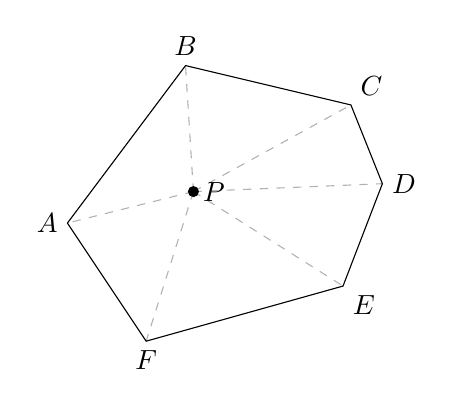
\begin{tikzpicture}
\coordinate (A1) at (0,2);
\coordinate (A2) at (1.5,4);
\coordinate (A3) at (3.6,3.5);
\coordinate (A4) at (4,2.5);
\coordinate (A5) at (3.5,1.2);
\coordinate (A6) at (1,0.5);
\coordinate (P) at (1.6,2.4);
\draw[dashed,color=black!30] (P)--(A1) (P)--(A2) (P)--(A3) (P)--(A4) (P)--(A5) (P)--(A6);
\draw (A1)node[left]{\(A\)}--(A2)node[above]{\(B\)}--(A3)node[above right]{\(C\)}--(A4)node[right]{\(D\)}--(A5)node[below right]{\(E\)}--(A6)node[below]{\(F\)}--(A1) (P)node[right]{\(P\)};
\fill (P)circle(2pt);
\end{tikzpicture}
\end{center}

\begin{theorem}
凸多边形的外角和为\(2\pi\).
\end{theorem}

\section{凸多面体}
\begin{theorem}[欧拉公式]
设凸多面体的顶点数、棱数、面数分别为\(V\)、\(E\)、\(F\),则有\[
V - E + F = 2.
\]
\end{theorem}

\begin{definition}
\textbf{正凸多面体}(简称\textbf{正多面体}),是指满足以下条件的凸多面体:
\begin{enumerate}
\item 正多面体的面由正多边形构成;
\item 正多面体的各个顶角相等;
\item 正多面体的各条棱长相等.
\end{enumerate}
\end{definition}

\begin{corollary}
正凸多面体只有5种:三四面体、正方体、正八面体、正十二面体、正二十面体.
\end{corollary}
